%
% File emnlp2020.tex
%
%% Based on the style files for ACL 2020, which were
%% Based on the style files for ACL 2018, NAACL 2018/19, which were
%% Based on the style files for ACL-2015, with some improvements
%%  taken from the NAACL-2016 style
%% Based on the style files for ACL-2014, which were, in turn,
%% based on ACL-2013, ACL-2012, ACL-2011, ACL-2010, ACL-IJCNLP-2009,
%% EACL-2009, IJCNLP-2008...
%% Based on the style files for EACL 2006 by 
%%e.agirre@ehu.es or Sergi.Balari@uab.es
%% and that of ACL 08 by Joakim Nivre and Noah Smith

\documentclass[11pt,a4paper]{article}
\usepackage[hyperref]{emnlp2020}
\usepackage{times}
\usepackage{latexsym}
\renewcommand{\UrlFont}{\ttfamily\small}

% This is not strictly necessary, and may be commented out,
% but it will improve the layout of the manuscript,
% and will typically save some space.
\usepackage{microtype}
\usepackage{amsmath,amsfonts}
\usepackage{bbm}
\usepackage{graphicx}
\usepackage{booktabs}
\usepackage{mathtools}
\usepackage{multirow}
\usepackage{siunitx}
%\aclfinalcopy % Uncomment this line for the final submission
%\def\aclpaperid{***} %  Enter the acl Paper ID here

%\setlength\titlebox{5cm}
% You can expand the titlebox if you need extra space
% to show all the authors. Please do not make the titlebox
% smaller than 5cm (the original size); we will check this
% in the camera-ready version and ask you to change it back.


%%%%%%%%%%%%%%%%%%%%%%%%%%%%%%%%%%%%%%%%%%%%%%%%%%%%%%%%%%%%%%%%%%%%%%%%%%%%%%%%
% latex functions
%%%%%%%%%%%%%%%%%%%%%%%%%%%%%%%%%%%%%%%%%%%%%%%%%%%%%%%%%%%%%%%%%%%%%%%%%%%%%%%%

\newcommand{\ltwo}[1]{\lVert{#1}\rVert}
\newcommand{\indicator}[1]{\mathbbm{1}\!\left[{#1}\right]}

\newcommand{\R}{\mathbb R}
\DeclareMathOperator*{\argmax}{arg\,max}
\DeclareMathOperator{\FindMostSimilar}{\texttt{FindMostSimilar}}
\DeclareMathOperator{\OddOneOut}{\texttt{OddOneOut}}
\DeclareMathOperator{\topk}{\texttt{Topk}}

\newcommand\BibTeX{B\textsc{ib}\TeX}
\special{papersize=210mm,297mm}

% Paper
\title{Instructions for EMNLP 2020 Proceedings}

\author{Nathan Stringham\\
  Affiliation / Address line 1 \\
  Affiliation / Address line 2 \\
  Affiliation / Address line 3 \\
  \texttt{email@domain} \\\And
  Mike Izbicki \\
  Affiliation / Address line 1 \\
  Affiliation / Address line 2 \\
  Affiliation / Address line 3 \\
  \texttt{email@domain} \\}

\date{}

\begin{document}
\maketitle
\begin{abstract}
%Use two-column format when you begin the abstract.
%Type the abstract at the beginning of the first column.
%The width of the abstract text should be smaller than the
%width of the columns for the text in the body of the paper by 0.6 cm on each side.
%Center the word \textbf{Abstract} in a 12 point bold font above the body of the abstract.
%The abstract should be a concise summary of the general thesis and conclusions of the paper.
%It should be no longer than 200 words.
%The abstract text should be in 10 point font.

The analogy task introduced by \cite{mikolov2013efficient} has become one of the most popular  methods for evaluating the quality of word embeddings;
 however, evidence suggests that analogies may not perform equally well across training contexts.
 Specifically, this method has proven non-trivial to adapt to languages beyond English and empirical evidence suggests that it requires large amounts of training data.
 As a result, those working in low resource or specialized settings have lacked a standard method to evaluate the quality of word embeddings.
 To address this problem, we propose two different intrinsic evaluation methods, which achieve greater performance sensitivity than the analogy task in low resource settings.
  We demonstrate the flexibility of these methods by using them to tune embeddings for $18$ low resource languages as well as the full list of unicode emojis.
   Furthermore, our methods are designed such that custom test sets can be developed semi-automatically in over $400$ different languages, which helps increase access for research in areas previously inhibited by low amounts of data.
\end{abstract}


%%% Copied this from other document
\section{Introduction}
\label{sec:intro}

%We need high quality word embeddings.
%Caveats: 
%- analogies were evaluated on english dataset only
%- word embeddings were trained in a resource rich scenario
%Still, analogies have become the go-to instrinsic evaluation method.
%- Many people who are trying to make good word embeddings in other languages have simply translated the google analogy set into their chosen language and then added a couple of new categories specific to their language. 
%- 3 CosMul and other attempts to modify the evaluation task...still buying in to the premise
%
%But, none of these approaches have really addressed the issue of not having enough data and difficulty of adapting the analogy task.
%
%People have talked about the weaknesses of the google analogy set, ie unbalanced between semantic and syntactic categories, mostly syntactic, when we usually care more about semantics.

% other stuff

The use of high quality distributed word embeddings has become important to achieve good performance on many tasks in natural language processing. One of the first and most popular methods for generating embeddings is word2vec introduced by \cite{mikolov2013efficient}.
 However, the popularity of word2vec was not won on the idea of distributed word embeddings alone, but also due to the high quality of their embeddings as evidenced by the ability to solve analogy relationships.
  Famously, they used the offset between pairs of vectors to reveal 'linguistic regularities' such as $\texttt{king} - \texttt{man} + \texttt{woman} = \texttt{queen}$. 
  Using this framework, \cite{mikolov2013efficient} formulated a $14$ category evaluation set consisting of a mix of semantic and syntactic relationships which was released alongside a set of pre-trained word vecors. 
  Since its release, the Google analogy test set has effectively become the gold standard for measuring embedding quality and spawned much work focused on using analogies to capture other linguistic regularities, increasing performance on the analogy test set, and translating the test set to be used with non-English languages. 
  At the same time, only small consideration has been given to areas where the analogy task either cannot be applied or fails to capture meaningful differences in quality between sets of embeddings.

\begin{figure}
\centering
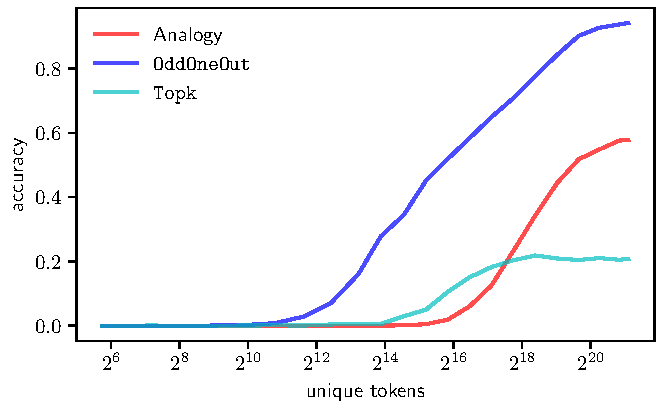
\includegraphics[width=1\columnwidth]{size_vs_acc.pdf} 
\caption{The plot above compares the regions of effectiveness for our evaluation metrics. 
The analogy task fails to measure change in accuracy of the embeddings until the number of unique words in the training dataset reaches  $2^{16}$, much later than both $\OddOneOut$ and $\topk$. 
Though $\OddOneOut$ seems the clear victor of these methods, experimentation in \ref{sec:experiments} shows that $\topk$ works better in some circumstances.}
\label{fig:data_vs_methods}
\end{figure}


Most work regarding word embeddings has been carried out in resource rich settings. 
In particular, the original word2vec embeddings were trained on a GoogleNews corpus containing 6 billion English tokens of which 783 million were unique \cite{mikolov2013efficient}.
 Unsurprisingly, greater amounts of training data leads to more accurate embeddings.
  But in reality, there are many domains in which this amount of data is impractical or even impossible to obtain. 
  Consider for example, a low resource language such as Telugu or a historical language like Latin.
  Furthermore, resource rich languages can quickly become low resource when considered from a specialized perspective.
   Those studying the evolution of language over time often require very specific corpora which in turn restricts the quantity of data. 

More recently, embeddings have even been generated for tokens that serve the purpose of words, but are not considered words in the traditional sense.
 The clearest example of these non-traditional embeddings is emoji, which have emerged as an important feature of natural language data in social media.
  In this setting it is unclear whether the analogy task should be applied and if so how to do so systematically and at scale.

In this paper, we demonstrate that the analogy task is not always suitable for evaluating quality of word embeddings,
 particularly when training resources are limited and when working in niche or specialized domains. 
 As a solution to this problem, we propose $\OddOneOut$ and $\topk$, two alternative evaluation methods which provide greater usability in low resource settings and are more general in nature.
  To further increase flexibility in deployment of embedding evaluation systems we also present Wikidata as a tool for generating test sets for these methods in up to $461$ languages. 


%\section{Contributions}
%\label{sec:contributions}
%\begin{itemize}
%	\item We show that the analogy task introduced by Mikolov et. al is not always suitable for evaluating the quality of word embeddings, particularly when embeddings are trained on small amounts of data.
%	\item We introduce two new methods for evaluating embeddings, $\OddOneOut$ and $\topk$.
%	\begin{itemize}
%		\item Use $\OddOneOut$ and $\topk$ to train emoji2vec model achieving comparable results to \citep{Eisner et al.}
%		\item These methods are more general (works for emojis and word embeddings)
%	\end{itemize}
%	\item We use wikidata to automatically generate test sets in multiple languages
%\end{itemize}

\section{Evaluation Methods}
\label{sec:method}
From a technical standpoint, our methods are quite simple and designed to be as generally applicable as possible.
 Both $\OddOneOut$ and $\topk$ require a test set which consists of groups of categories where each category contains words that are semantically similar. 
 The $\OddOneOut$ method seeks to identify the word that does not belong when presented with a group of words.
  For a given word, $\topk$ finds the k most similar words according to the model and compares them to words that belong to the semantic category from which the word was chosen.


We now formalize the methods. 
Assume that there are $m$ categories, that each category has $n$ words, that there are $v$ total words in the vocabulary, and that the words are embedded into $\R^d$.
Let $c_{i,j}$ be the $j$th word in category $i$,
and let $C_i = \{c_{i,1}, c_{i,2}, ..., c_{i,n}\}$ be the $i$th category.

\subsection{The $\topk$ method}
Let $\FindMostSimilar(k,w)$ return the $k$ most similar words in the vocabulary to $w$.
We define the $\topk$ score for class $i$ to be
\begin{equation}
    \topk(k,i) = \frac{1}{n}\sum_{j=1}^n \frac{1}{k}\sum_{\mathrlap{x \in \FindMostSimilar(k, c_{i,j})}} \indicator{x \in C_i}
\end{equation}
and the $\topk$ score for the entire evaluation set to be
\begin{equation}
    \topk(k) = \frac{1}{m}\sum_{i=1}^m \topk(k,i)
    .
\end{equation}

The runtime of $\FindMostSimilar$ is $O(dvk)$.\footnote{
    We use gensim's implementation of $\FindMostSimilar$,
    which uses the naive loop strategy for computing the nearest neighbor.
    Data structures like the $k$d-tree or cover tree could potentially be used to speed up this search,
    but we did not find such data structures necessary.
}
So the runtime of $\topk(k,i)$ is $O(dnk^2v)$
and the runtime of $\topk(k)$ is $O(dnmk^2v)$.
Typically $k$ is small (we recommend $k=3$ in our experiments),
and so the runtime is linear in all of the interesting parameters.
In particular, it is linear in both the size of our input data and evaluation set.

\subsection{The $\OddOneOut$ method}
Define the $\OddOneOut$ score of a set $S$ with $k$ words with respect to a word $w\not\in S$ as

%\begin{equation}
%    \OddOneOut(S,w) = \indicator{w = \hat w},
%\end{equation}
%where
%\begin{equation}
%    \hat w = \argmax_{x \in S\cup\{w\}} \ltwo{x - \mu}
%    \quad
%    \text{and}
%    \quad
%    \mu = \frac1{k+1}\bigg(w + \sum_{i=1}^k{s_i}\bigg)
%    .
%\end{equation}

\begin{equation}
    \OddOneOut(S,w) = \indicator{w = \hat w},
\end{equation}
where
\begin{equation}
    \hat w = \argmax_{x \in S\cup\{w\}} \ltwo{x - \mu}
\end{equation}
\begin{equation}
    %\quad
    \text{and}
    \quad
    \mu = \frac1{k+1}\bigg(w + \sum_{i=1}^k{s_i}\bigg)
    .
\end{equation}


We define the $k$th order $\OddOneOut$ score of a category $i$ to be
\begin{equation}
    \OddOneOut(k,i) = \frac 1 {|P|} \sum_{\mathclap{(S,w) \in P}} \OddOneOut(S,w)
\end{equation}
where
\begin{equation}
    P = \{ (S, w) : S \text{~is a combination of $k$ words from $C_i$}, \text{and~} w \in V-C_i \}
    .
    \label{eq:P}
\end{equation}
In Equation \eqref{eq:P} above,
the total number of values that $S$ can take is ${n \choose k} = O(n^k)$,
and the total number of values that $w$ can take is $O(v)$,
so $|P| = O(n^kv)$.
Finally, we define the $k$-th order $\OddOneOut$ score of the entire evaluation set to be
\begin{equation}
    \OddOneOut(k) = \frac 1 m \sum_{i=1}^m \OddOneOut(k,i)
    .
\end{equation}

The runtime of $\OddOneOut(S,w)$ is $O(dk)$.
So the runtime of $\OddOneOut(k,i)$ is $O(dkn^kv)$ and the runtime of $\OddOneOut(k)$ is $O(dkmn^kv)$.

Comparing the runtimes of $\OddOneOut(k)$ and $\topk(k)$, we can see that $\OddOneOut(k)$ is a factor of $O(m^{k-1}k^{-1})$ slower.
In real world applications, $m >\!\!> k$, and so $\OddOneOut$ will take considerably more time to compute.
In particular, the Mikolov test evaluations in Section \ref{sec:experiments} below use $m=50$ and $k=3$,
so the $\OddOneOut(k)$ score takes approximately 800x longer to compute.

\section{Experiments}
\label{sec:experiments}
\subsection{English Experiments}

%\showthe\columnwidth

First we seek to illustrate how performance on the analogy task, $\OddOneOut$, and $\topk$ relates to size of the training corpus. 
Since the original GoogleNews dataset is not available to the public we instead use a 2017 dump from English Wikipedia readily available through the gensim library.
 This dataset consists of 2 billion tokens with 2 million unique.
 While not quite as large as GoogleNews, it serves as a good proxy for the high resource setting in English.

We test the relationship between amount of training data and embedding performance on the analogy task by training a series of models on subsets of our corpus.
 We train our first model with a subset containing $2^{6}$ unique tokens and double the number of unique tokens for each subsequent model until all tokens are used. 
 Since the Wikipedia corpus is alphabetized by article, a sequential streaming of the data would introduce bias. The smallest models would only be trained on content related to articles near the beginning of the alphabet.
 This is a problem because larger models would have the benefit of both greater amounts of data as well as a greater contextual variety of data compared to smaller ones. 
 To mitigate this bias we use a linear congruential generator to randomly stream the training data in a way that is reproducible. 
 Thus, in addition to mitigating model bias tied to the content of training data, our random generator also ensures that each model uses a subset of the training data of models larger than it.
  In total, we train $25$ word2vec models with the following fixed set of hyperparameters: dimension = $100$, epochs = $1$, learning rate = $.025$, window size = $5$, min count = $5$.

To calculate accuracies we use the Google analogy test set to which is easily adapted for use with $\OddOneOut$ and $\topk$ by splitting each relationship pair into two separate categories.

Figure \ref{fig:data_vs_methods} shows the results of the evaluation of these models on three intrinsic tasks-- \texttt{Analogy}, \texttt{OddOneOut}, and \texttt{Topk}.
 We see that for the various tasks both \texttt{OddOneOut} and \texttt{Topk} start to see an increase in performance with roughly $32x$ less data compared to \texttt{Analogy}. 
 In addition, though the shapes are roughly similar, the curve for \texttt{OddOneOut} and \texttt{Topk} have steeper slopes before plateauing, 
 indicating a greater sensitivity to amount of data.
  Overall, these findings suggest that in the low resource scenarios, the analogy task does will not always provide adequate intrinsic evaluation for word embeddings,
  especially compared to these simpler methods.


\begin{figure*}
\centering
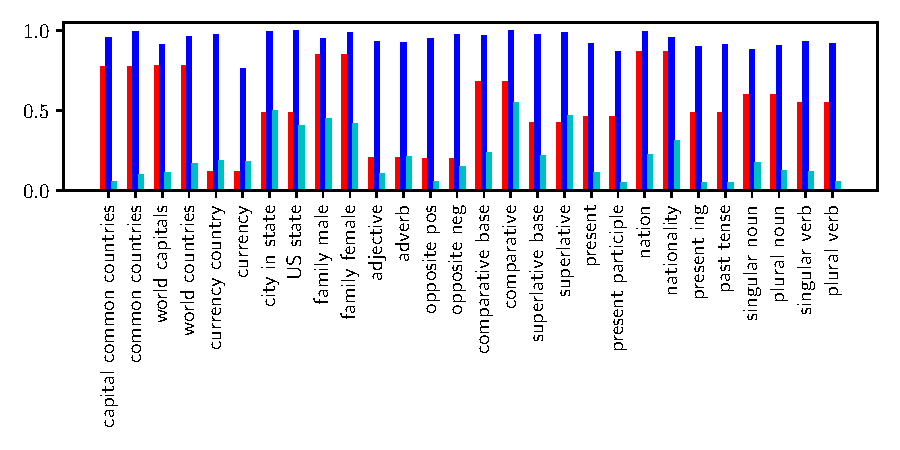
\includegraphics{cross_cat_acc.pdf} 
\caption{The methods perform better on some categories than others. $\topk$  seems to excel in categories that are more homogenous like 'family female',
 while analogies seem to work best with geographical relationships.
  Note that in adapting the Google analogy set to work with our methods required splitting each relationship pair into two separate categories. 
  As a result the analogy score for a given relationship is shown twice;
   one bar in each of the categories that make up the pair.}
\label{fig:data_vs_methods}
\end{figure*}


\subsection{Emoji Experiments}
\begin{figure*}
\centering
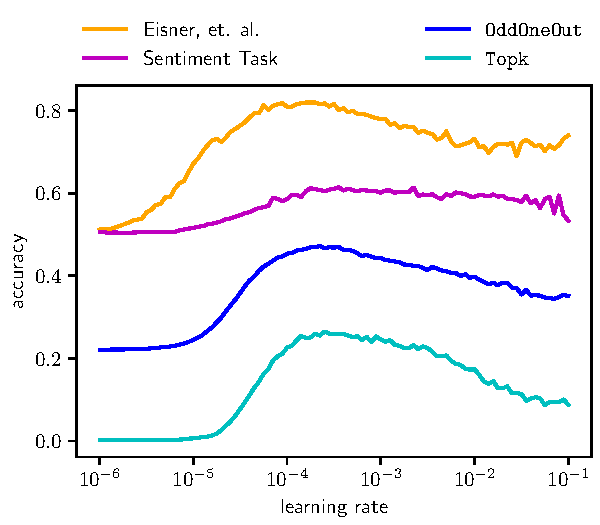
\includegraphics{emoji_exp.pdf} 
\caption{This figures shows the tuning of emoji embeddings across different learning learning rates where the max accuracy for each metric is marked with a point.
 Both $\topk$ and $\OddOneOut$ follow the shape of \cite{eisner2016emoji2vec} area under the curve and accuracy metrics.
 Our methods lead us to select essentially the same hyperparameters as \cite{eisner2016emoji2vec} and reproduced results on the downstream task.}
\label{fig:emoji}
\end{figure*}

In addition to performing poorly as an evaluation metric in low resource circumstances,
the analogy task does not easily generalize beyond traditional word embeddings.
One example of this where this is prevalent is in the case of emoji embeddings.
With the rise of social media data, a good amount of semantic data has been showed to be captured in the form of emojis. 
In 2016 \cite{eisner2016emoji2vec} introduce pretrained emoji embeddings known as emoji2vec. 
In their paper, \cite{eisner2016emoji2vec} mention the analogy task as a way of evaluating the quality of their embeddings;
 however, the analogy task is not easily adaptable to this specialized domain.
 As a result they were forced to settle for a qualitative analysis of small number of analogy relationships that were translatable.
 In order to quantitatively evaluate and tune their set of emoji embeddings, \cite{eisner2016emoji2vec} develop their own 'emoji-description classification' method  which required the creation of a test set with manually labeled emotion-description pairs.

The simple and general design of our methods allows them to be easily adapted to intrinsically evaluate emoji embeddings.
We demonstrate this by training our own emoji embeddings using \cite{eisner2016emoji2vec} code with $\OddOneOut$ and $\topk$ as the fine tuning metric.
The semantic categories of emojis are trivial to generate from unicode's full emoji list\footnote{\url{https://unicode.org/Public/emoji/13.0/emoji-test.txt}} 

In addition to intrinsic evaluation of emoji2vec with their custom method, \cite{eisner2016emoji2vec} also deploy their vectors in a downstream sentiment analysis of tweets.
We verify the performance of our tuned emoji embeddings by also evaluating performance on this same sentiment analysis task.
Figure \ref{fig:emoji} shows the results of evaluation, we find that our embeddings were able to reproduce \cite{eisner2016emoji2vec} performance on the downstream task.

\subsection{Automatic Test Set Generation with Wikidata}

One of the most difficult and time consuming steps in the process of generating of high quality word embeddings is the creation of a comprehensive test set.
 Consequently, one of the biggest advantages of the $\OddOneOut$ and $\topk$ methods is that compatible test sets can be semi-automatically generated in hundreds of languages.
This is possible using Wikidata. 
This publicly available SPARQL database contains a comprehensive structure of the semantic content contained in Wikipedia
along with its relationship to other items.
Simple queries constructed using the Wikidata Query Service can be used to return semantic categories of words that can be included in a test set.

Using Wikidata we were able to reconstruct all of the semantic categories contained within the Google analogy set with the option of greater customization and more categories.
 Additionally, Wikidata supports the translation of queried items into 461 languages, allowing test sets to easily be converted between languages.
  Though not all items have translated labels in all 461 languages, support is quite extensive and will only get better. 

One of the disadvantages of using Wikidata is that syntactic categories are much harder to construct;
 however, since semantic categories are usually more difficult to generate 
 and require more arbitrary decisions this approach is still very valuable.

\subsection{Classical Languages Experiments}

% Improved Table - Combined Score
\begin{table*}[t]
\centering
\scalebox{.55}{
\begin{tabular}{l|llrr|llrrrrl|rrr}
\toprule
\multicolumn{5}{c}{\bf Corpus} & \multicolumn{7}{c}{\bf Parameters} & \multicolumn{3}{c}{\bf Scores} \\
\midrule
& Language & Test Set & Tokens & Unique Tokens & Model & Type & Dim & Window & LR & Min Count & Lemma & $\OddOneOut$ & $\topk$ & \texttt{Combined} \\
\midrule
    
    \multirow{2}{*}{Hellenic}& greek & ancient greek & \num{37868209} & \num{1877574} & w2v & cbow & 40 & 9 & -1 & 4 & False & 1140 & 8 & 17.86\\
    & greek & modern greek & \num{37868209} & \num{1877574} & fast & sg & 90 & 7 & -1 & 5 & True & 300 & 9 & 19.36\\  
    \midrule
    \multirow{2}{*}{Italic}&latin & latin & \num{17777429} & \num{470790} & w2v & cbow & 50 & 10 & -1 & 7 & False & 2748 & 48 & 96.28\\ 
    &old french  & french & \num{68741} & \num{8343} &  fast & sg & 250 & 6 & -1 & 8  & False & 1 & 7 & 3.20\\
    \midrule
    \multirow{5}{*}{Germanic}&middle english & english (old) & \num{7048144} & \num{314527} & fast & sg & 90 & 5 & -1 & 7 & False & 239 & 7 & 15.48 \\
    &middle high german & german & \num{2090954} & \num{60674} & fast & cbow & 15 & 6 & -1 & 3 & False & 9 & 19 & 13.33 \\
    &old english  & english (old) & \num{104011} & \num{33018} & fast & cbow & 425 & 3 & -1 & 3 & True & 0 & 1  & 1.33 \\
    &old norse & icelandic & \num{458377} & \num{59186} & w2v & cbow & 60 & 10 & -1 & 3 & False & 968 & 2 & 5.98 \\
    &old swedish & swedish & \num{1297740} & \num{116374} &  fast & sg & 50 & 8 & -1 & 5 & False & 50 & 1 & 3.85 \\
    \midrule
    \multirow{8}{*}{Indo-Aryan}&bengali & bengali & \num{5539} & \num{2323} & fast & cbow & 15 & 3 & -1 & 4 & False & 0 & 2 & 1.50 \\
    &gujarati & gujarati & \num{1813} & \num{1140} & fast & sg & 80 & 3 & -1 & 5 & False & 0 & 7 & 1.78 \\
    &hindi & hindi& \num{587655} & \num{55483} & fast & cbow & 45 & 4 & -1 & 8 & False & 263 & 2 & 5.93\\
    &malayalam & malayalam& \num{9235} & \num{5405} & - & - & - & - & - & - & - & - & - & - \\
    &marathi & marathi & \num{797926} & \num{96778} & w2v & sg & 400 & 4 & -1 & 6 & False & 342 & 1 & 3.98 \\
    &punjabi & punjabi & \num{1024075} & \num{31343} & fast & sg & 50 & 8 & -1 & 5 & False & 0 & 1 & 1.3 \\
    &sanskrit & sanskrit & \num{4042204} & \num{896480} & w2v & sg & 35 & 9 & -1 & 10 & False & 1530 & 1 & 3.99\\
    &telugu & telugu & \num{537673} & \num{276330} &  w2v & cbow & 60 & 10 & -1 & 3 & False & 50 & 0 & 1.96 \\
    \midrule
    \multirow{2}{*}{Semitic}&classical arabic & arabic& \num{81306} & \num{20493} & - & - & - & - & - & - & - & - & - & - \\
    &hebrew & hebrew & \num{41378460} & \num{893512} & fast & sg & 30 & 4 & -1 & 3 & False & 1098 & 6 & 13.91 \\  
\bottomrule
\end{tabular}
}
\caption{The table above provides details for the best model trained for languages supported by CLTK.
Following a tuning process, models were chosen by their $\texttt{Combined Score}$
which is calculated as the harmonic mean of $\topk$ and $\OddOneOut$.
It is important to note that the absolute score for our evaluation metrics are not important in and of themselves,
rather they are important as indicators of a change in embedding quality that the analogy task would fail to show.
To emphasize this, we have reported the raw number of correct answers for each metric.
Using $\OddOneOut$ and $\topk$ allows us to tune models trained on corpora with unique token counts in the thousands instead of the millions.}
\label{table:language}
\end{table*}

An obvious application of $\OddOneOut$ and $\topk$ is in training models for under-resourced languages. 
The Classical Language Toolkit (CLTK) \cite{johnson2014} is one such ongoing project supporting nlp for various classical, low resource, and often historical languages.
To confirm the efficacy of our methods in the low resource setting, we train and tune word embeddings on all languages supported by the Classical Language Toolkit which contain at least one downloadable corpus and a tokenization tool. 
In total this leaves us with $18$ low resource languages.

For each language we preprocess all corpora available through CLTK, using their normalization and tokenization tools where appropriate. 
We then perform a randomized grid search over the key model parameters consisting of 100 samples. 
The key hyperparameters we searched over can be found in Table \ref{table:language}. 
After training the model we perform an intrinsic evaluation for the embeddings on the corresponding language specific test set 
and pick the model that had the highest \texttt{Combined Score} 
which is calculated as the harmonic mean of $\OddOneOut$ and $\topk$.

Although the parameter combinations searched over for each language were the same,
the best model for each language contained a unique set of parameters. 
This supports the need for an intrinsic tuning method for word embeddings so that highest performance can be achieved. 
The tuning results in Table \ref{table:language} also seem to indicate that fastText models perform better than word2vec in low resource scenarios 
 due to the training of n-grams.


%Biblical
\section{Multilingual Content Analysis}
Aside from intrinsic evaluation, our methods can be leveraged as a qualitative downstream task we call multilingual content analysis.
The goal of the task is to determine the degree to which some concept or category is captured by a set of word embeddings. 
We implement this by using Wikidata to construct $3$ categories of interest--Biblical Figures, Facets of Hinduism, and Facets of Buddhism--and then evaluate them using $\OddOneOut$ and $\topk$. 
The performance on this task demonstrates the degree to which our models understand the semantics of the chosen topics 
and provides insight regarding the content they were trained on.

With intentionally selected categories we are able draw out the differences in content between the different language models
that in many cases matches our intuition. 
By evaluating on a category of biblical figures we see highest performance from the Hebrew and Latin models followed by other European languages; 
whereas Facets of Buddhism and Facets of Hinduism see high performance from the Indic language models.

Perhaps more interesting, this downstream task also gives rise to circumstances in which $\topk$ performance exceeded $\OddOneOut$. 
In some cases (like Middle High German on Biblical Figures) $\topk$ merely surpasses $\OddOneOut$ 
and in others (such as Gujarati on Facets of Hinduism) it is the only metric to achieve a performance score. 
It is likely that a complex interaction between the model and the category being evaluated on can result in either method achieving better performance, 
thus it is valuable to have both methods at our disposal. 
Since this exact relationship is still not fully understood we tune and evaluate models using both metrics 
and compute the harmonic mean to choose the most accurate model.

\begin{figure*}
\centering
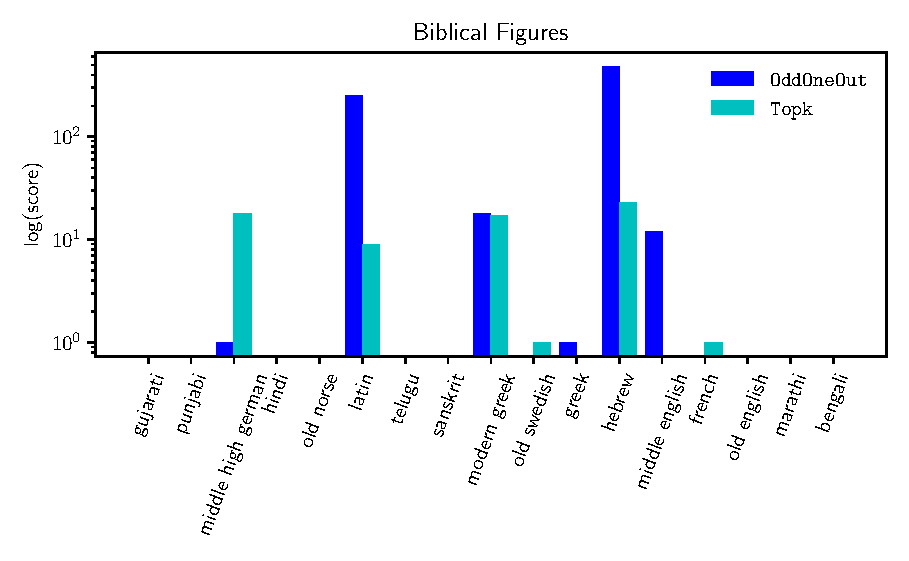
\includegraphics{biblical-raw.pdf} 
\caption{High performance on the Biblical Figures category indicates some level of biblical influence via the corpus. 
Interestingly, we see that greek embeddings optimized on the Modern Greek test set significantly outperformed the embeddings optimized for the Ancient Greek. 
This matches our intuition that things of a biblical nature have had a greater influence on Modern Greek than Ancient Greek.}
\label{fig:biblicall}
\end{figure*}

%Buddhism
\begin{figure*}
\centering
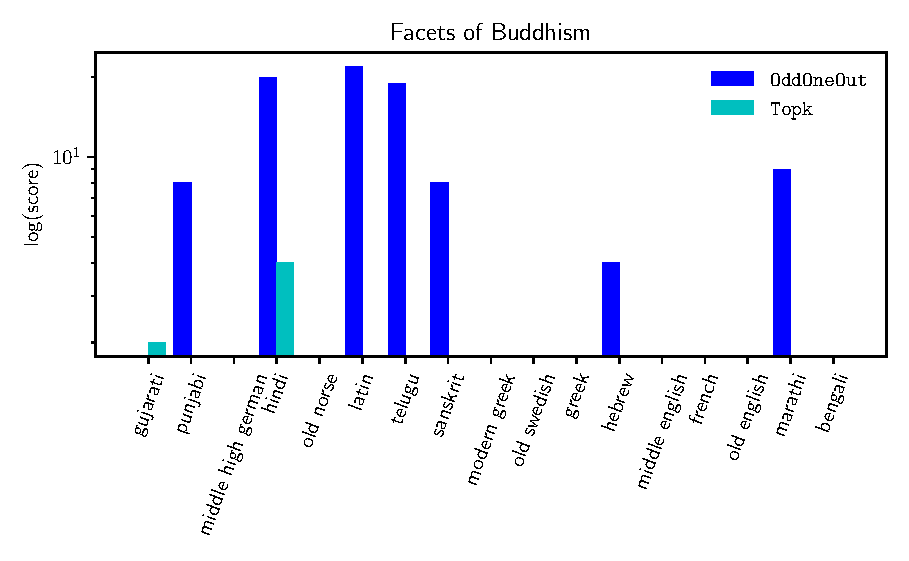
\includegraphics{buddhism-raw.pdf} 
\caption{Though many of the Indic language embeddings performed well on the Facets of Buddhism, 
surprisingly so did our Latin and Hebrew embeddings. 
This leads us to believe that some Buddhist concepts and words are shared by corpora spanning languages as diverse as Hebrew, Latin, and Hindi. 
At the same time, it should also be noted that Latin and Hebrew were two of the largest models trained compared to other classical languages and thus also likely benefit from greater resource richness.}
\label{fig:buddhism}
\end{figure*}

%Hinduism
\begin{figure*}
\centering
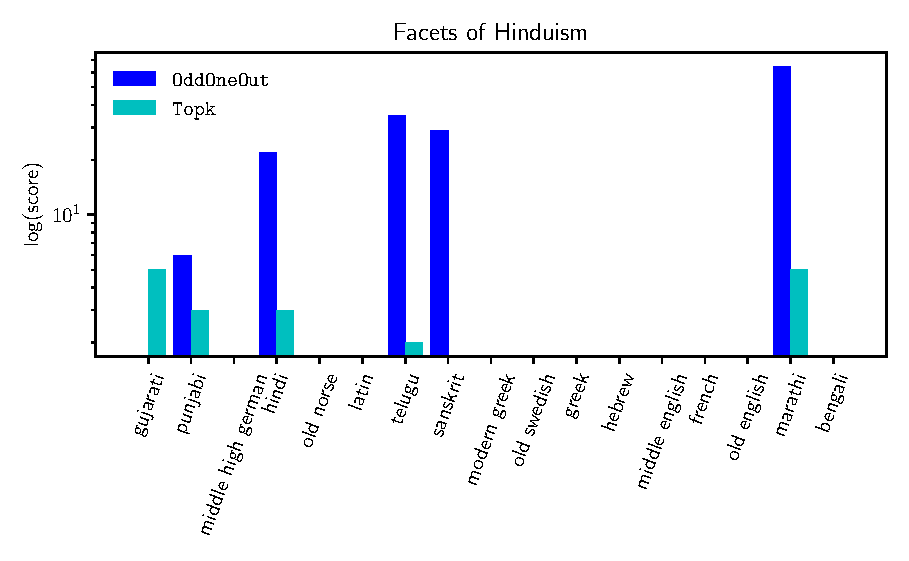
\includegraphics{hinduism-raw.pdf} 
\caption{Similar to Figure \ref{fig:biblical} we see languages more closely related to the topic of the category achieving better performance, in this case primarily the Indic languages. 
Interstingly, our Bengali embeddings performed poorly on this category suggesting that the corpus did not refer heavily to the Hindu context}
\label{fig:hinduism}
\end{figure*}

%animals
%\begin{figure*}
%\centering
%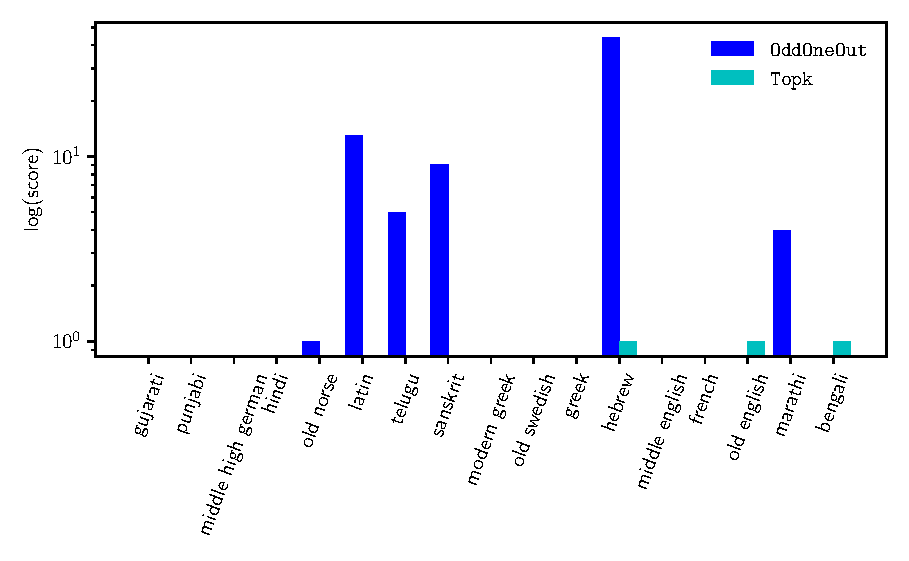
\includegraphics{animals-raw.pdf} 
%\caption{}
%\label{fig:multilingual}
%\end{figure*}

\section{Acknowledgements}
\label{sed:acknowledgements}

\section{Related Work}
\label{sec:related}



%\section{Related Work}
%\label{sec:related}



%\subsection{Nate}
%
%Look at the way these papers run experiments:
%
%\cite{tifrea2018poincar,meng2019spherical}
%
%Datasets at: \url{https://aclweb.org/aclwiki/Similarity_(State_of_the_art)}
%
%Use wikidata to automatically generate classes: https://www.wikidata.org/wiki/Q43689 
%https://pywikidata.readthedocs.io/en/latest/
%
%wikidata church fathers in latin: \url{https://query.wikidata.org/#SELECT%20%3Fperson%20%3FpersonLabel%0AWHERE%20%7B%0A%20%20%3Fperson%20wdt%3AP361%20wd%3AQ182603.%0A%20%20SERVICE%20wikibase%3Alabel%20%7B%20bd%3AserviceParam%20wikibase%3Alanguage%20%22la%22.%20%7D%0A%7D}
%
%SPARQL Tutorial: \url{https://www.wikidata.org/wiki/Wikidata:SPARQL_tutorial}
%
%Can we use wikidata to automatically generate good evaluations?
%
%\section{Discussion}
%\label{sec:discussion}



%%% End of my stuff 


%\section{Electronically-available resources}
%
%ACL provides this description and accompanying style files at
%\begin{quote}
%\url{https://2020.emnlp.org/files/emnlp2020-templates.zip}
%\end{quote}
%We strongly recommend the use of these style files, which have been appropriately tailored for the EMNLP 2020 proceedings.
%
%\paragraph{\LaTeX-specific details:}
%The templates include the \LaTeX2e{} source (\texttt{\small emnlp2020.tex}),
%the \LaTeX2e{} style file used to format it (\texttt{\small emnlp2020.sty}),
%an ACL bibliography style (\texttt{\small acl\_natbib.bst}),
%an example bibliography (\texttt{\small emnlp2020.bib}),
%and the bibliography for the ACL Anthology (\texttt{\small anthology.bib}).
%
%
%\section{Length of Submission}
%\label{sec:length}
%
%The conference accepts submissions of long papers and short papers.
%Long papers may consist of up to eight (8) pages of content plus unlimited pages for references.
%Upon acceptance, final versions of long papers will be given one additional page -- up to nine (9) pages of content plus unlimited pages for references -- so that reviewers' comments can be taken into account.
%Short papers may consist of up to four (4) pages of content, plus unlimited pages for references.
%Upon acceptance, short papers will be given five (5) pages in the proceedings and unlimited pages for references. 
%For both long and short papers, all illustrations and tables that are part of the main text must be accommodated within these page limits, observing the formatting instructions given in the present document.
%Papers that do not conform to the specified length and formatting requirements are subject to be rejected without review.
%
%The conference encourages the submission of additional material that is relevant to the reviewers but not an integral part of the paper.
%There are two such types of material: appendices, which can be read, and non-readable supplementary materials, often data or code.
%Additional material must be submitted as separate files, and must adhere to the same anonymity guidelines as the main paper.
%The paper must be self-contained: it is optional for reviewers to look at the supplementary material.
%Papers should not refer, for further detail, to documents, code or data resources that are not available to the reviewers.
%Refer to Appendices~\ref{sec:appendix} and \ref{sec:supplemental} for further information. 
%
%Workshop chairs may have different rules for allowed length and whether supplemental material is welcome.
%As always, the respective call for papers is the authoritative source.
%
%
%\section{Anonymity}
%As reviewing will be double-blind, papers submitted for review should not include any author information (such as names or affiliations). Furthermore, self-references that reveal the author's identity, \emph{e.g.},
%\begin{quote}
%We previously showed \citep{Gusfield:97} \ldots
%\end{quote}
%should be avoided. Instead, use citations such as 
%\begin{quote}
%\citet{Gusfield:97} previously showed\ldots
%\end{quote}
%Please do not use anonymous citations and do not include acknowledgements.
%\textbf{Papers that do not conform to these requirements may be rejected without review.}
%
%Any preliminary non-archival versions of submitted papers should be listed in the submission form but not in the review version of the paper.
%Reviewers are generally aware that authors may present preliminary versions of their work in other venues, but will not be provided the list of previous presentations from the submission form.
%
%Once a paper has been accepted to the conference, the camera-ready version of the paper should include the author's names and affiliations, and is allowed to use self-references.
%
%\paragraph{\LaTeX-specific details:}
%For an anonymized submission, ensure that {\small\verb|\aclfinalcopy|} at the top of this document is commented out, and that you have filled in the paper ID number (assigned during the submission process on softconf) where {\small\verb|***|} appears in the {\small\verb|\def\aclpaperid{***}|} definition at the top of this document.
%For a camera-ready submission, ensure that {\small\verb|\aclfinalcopy|} at the top of this document is not commented out.
%
%
%\section{Multiple Submission Policy}
%
%EMNLP 2020 will not consider any paper that is under review in a journal or another conference at the time of submission, and submitted papers must not be submitted elsewhere during the EMNLP 2020 review period. This policy covers all refereed and archival conferences and workshops (e.g., COLING, NeurIPS, ACL workshops). For example, a paper under review at an ACL workshop cannot be dual-submitted to EMNLP 2020. The only exception is that a paper can be dual-submitted to both EMNLP 2020 and an EMNLP workshop which has its submission deadline falling after our original notification date of August 8, 2020. In addition, we will not consider any paper that overlaps significantly in content or results with papers that will be (or have been) published elsewhere. 
%
%Authors submitting more than one paper to EMNLP 2020 must ensure that their submissions do not overlap significantly ($>25$\%) with each other in content or results.
%
%\section{Formatting Instructions}
%
%Manuscripts must be in two-column format.
%Exceptions to the two-column format include the title, authors' names and complete addresses, which must be centered at the top of the first page, and any full-width figures or tables (see the guidelines in Section~\ref{ssec:title-authors}).
%\textbf{Type single-spaced.}
%Start all pages directly under the top margin.
%The manuscript should be printed single-sided and its length should not exceed the maximum page limit described in Section~\ref{sec:length}.
%Pages should be numbered in the version submitted for review, but \textbf{pages should not be numbered in the camera-ready version}.
%
%\paragraph{\LaTeX-specific details:}
%The style files will generate page numbers when {\small\verb|\aclfinalcopy|} is commented out, and remove them otherwise.
%
%
%\subsection{File Format}
%\label{sect:pdf}
%
%For the production of the electronic manuscript you must use Adobe's Portable Document Format (PDF).
%Please make sure that your PDF file includes all the necessary fonts (especially tree diagrams, symbols, and fonts with Asian characters).
%When you print or create the PDF file, there is usually an option in your printer setup to include none, all or just non-standard fonts.
%Please make sure that you select the option of including ALL the fonts.
%\textbf{Before sending it, test your PDF by printing it from a computer different from the one where it was created.}
%Moreover, some word processors may generate very large PDF files, where each page is rendered as an image.
%Such images may reproduce poorly.
%In this case, try alternative ways to obtain the PDF.
%One way on some systems is to install a driver for a postscript printer, send your document to the printer specifying ``Output to a file'', then convert the file to PDF.
%
%It is of utmost importance to specify the \textbf{A4 format} (21 cm x 29.7 cm) when formatting the paper.
%Print-outs of the PDF file on A4 paper should be identical to the hardcopy version.
%If you cannot meet the above requirements about the production of your electronic submission, please contact the publication chairs as soon as possible.
%
%\paragraph{\LaTeX-specific details:}
%PDF files are usually produced from \LaTeX{} using the \texttt{\small pdflatex} command.
%If your version of \LaTeX{} produces Postscript files, \texttt{\small ps2pdf} or \texttt{\small dvipdf} can convert these to PDF.
%To ensure A4 format in \LaTeX, use the command {\small\verb|\special{papersize=210mm,297mm}|}
%in the \LaTeX{} preamble (below the {\small\verb|\usepackage|} commands) and use \texttt{\small dvipdf} and/or \texttt{\small pdflatex}; or specify \texttt{\small -t a4} when working with \texttt{\small dvips}.
%
%\subsection{Layout}
%\label{ssec:layout}
%
%Format manuscripts two columns to a page, in the manner these
%instructions are formatted.
%The exact dimensions for a page on A4 paper are:
%
%\begin{itemize}
%\item Left and right margins: 2.5 cm
%\item Top margin: 2.5 cm
%\item Bottom margin: 2.5 cm
%\item Column width: 7.7 cm
%\item Column height: 24.7 cm
%\item Gap between columns: 0.6 cm
%\end{itemize}
%
%\noindent Papers should not be submitted on any other paper size.
%If you cannot meet the above requirements about the production of your electronic submission, please contact the publication chairs above as soon as possible.
%
%\subsection{Fonts}
%
%For reasons of uniformity, Adobe's \textbf{Times Roman} font should be used.
%If Times Roman is unavailable, you may use Times New Roman or \textbf{Computer Modern Roman}.
%
%Table~\ref{font-table} specifies what font sizes and styles must be used for each type of text in the manuscript.
%
%\begin{table}
%\centering
%\begin{tabular}{lrl}
%\hline \textbf{Type of Text} & \textbf{Font Size} & \textbf{Style} \\ \hline
%paper title & 15 pt & bold \\
%author names & 12 pt & bold \\
%author affiliation & 12 pt & \\
%the word ``Abstract'' & 12 pt & bold \\
%section titles & 12 pt & bold \\
%subsection titles & 11 pt & bold \\
%document text & 11 pt  &\\
%captions & 10 pt & \\
%abstract text & 10 pt & \\
%bibliography & 10 pt & \\
%footnotes & 9 pt & \\
%\hline
%\end{tabular}
%\caption{\label{font-table} Font guide. }
%\end{table}
%
%\paragraph{\LaTeX-specific details:}
%To use Times Roman in \LaTeX2e{}, put the following in the preamble:
%\begin{quote}
%\small
%\begin{verbatim}
%\usepackage{times}
%\usepackage{latexsym}
%\end{verbatim}
%\end{quote}
%
%
%\subsection{Ruler}
%A printed ruler (line numbers in the left and right margins of the article) should be presented in the version submitted for review, so that reviewers may comment on particular lines in the paper without circumlocution.
%The presence or absence of the ruler should not change the appearance of any other content on the page.
%The camera ready copy should not contain a ruler.
%
%\paragraph{Reviewers:}
%note that the ruler measurements may not align well with lines in the paper -- this turns out to be very difficult to do well when the paper contains many figures and equations, and, when done, looks ugly.
%In most cases one would expect that the approximate location will be adequate, although you can also use fractional references (\emph{e.g.}, this line ends at mark $295.5$).
%
%\paragraph{\LaTeX-specific details:}
%The style files will generate the ruler when {\small\verb|\aclfinalcopy|} is commented out, and remove it otherwise.
%
%\subsection{Title and Authors}
%\label{ssec:title-authors}
%
%Center the title, author's name(s) and affiliation(s) across both columns.
%Do not use footnotes for affiliations.
%Place the title centered at the top of the first page, in a 15-point bold font.
%Long titles should be typed on two lines without a blank line intervening.
%Put the title 2.5 cm from the top of the page, followed by a blank line, then the author's names(s), and the affiliation on the following line.
%Do not use only initials for given names (middle initials are allowed).
%Do not format surnames in all capitals (\emph{e.g.}, use ``Mitchell'' not ``MITCHELL'').
%Do not format title and section headings in all capitals except for proper names (such as ``BLEU'') that are
%conventionally in all capitals.
%The affiliation should contain the author's complete address, and if possible, an electronic mail address.
%
%The title, author names and addresses should be completely identical to those entered to the electronical paper submission website in order to maintain the consistency of author information among all publications of the conference.
%If they are different, the publication chairs may resolve the difference without consulting with you; so it is in your own interest to double-check that the information is consistent.
%
%Start the body of the first page 7.5 cm from the top of the page.
%\textbf{Even in the anonymous version of the paper, you should maintain space for names and addresses so that they will fit in the final (accepted) version.}
%
%
%\subsection{Abstract}
%Use two-column format when you begin the abstract.
%Type the abstract at the beginning of the first column.
%The width of the abstract text should be smaller than the
%width of the columns for the text in the body of the paper by 0.6 cm on each side.
%Center the word \textbf{Abstract} in a 12 point bold font above the body of the abstract.
%The abstract should be a concise summary of the general thesis and conclusions of the paper.
%It should be no longer than 200 words.
%The abstract text should be in 10 point font.
%
%\subsection{Text}
%Begin typing the main body of the text immediately after the abstract, observing the two-column format as shown in the present document.
%
%Indent 0.4 cm when starting a new paragraph.
%
%\subsection{Sections}
%
%Format section and subsection headings in the style shown on the present document.
%Use numbered sections (Arabic numerals) to facilitate cross references.
%Number subsections with the section number and the subsection number separated by a dot, in Arabic numerals.
%
%\subsection{Footnotes}
%Put footnotes at the bottom of the page and use 9 point font.
%They may be numbered or referred to by asterisks or other symbols.\footnote{This is how a footnote should appear.}
%Footnotes should be separated from the text by a line.\footnote{Note the line separating the footnotes from the text.}
%
%\subsection{Graphics}
%
%Place figures, tables, and photographs in the paper near where they are first discussed, rather than at the end, if possible.
%Wide illustrations may run across both columns.
%Color is allowed, but adhere to Section~\ref{ssec:accessibility}'s guidelines on accessibility.
%
%\paragraph{Captions:}
%Provide a caption for every illustration; number each one sequentially in the form:
%``Figure 1. Caption of the Figure.''
%``Table 1. Caption of the Table.''
%Type the captions of the figures and tables below the body, using 10 point text.
%Captions should be placed below illustrations.
%Captions that are one line are centered (see Table~\ref{font-table}).
%Captions longer than one line are left-aligned (see Table~\ref{tab:accents}).
%
%\begin{table}
%\centering
%\begin{tabular}{lc}
%\hline
%\textbf{Command} & \textbf{Output}\\
%\hline
%\verb|{\"a}| & {\"a} \\
%\verb|{\^e}| & {\^e} \\
%\verb|{\`i}| & {\`i} \\ 
%\verb|{\.I}| & {\.I} \\ 
%\verb|{\o}| & {\o} \\
%\verb|{\'u}| & {\'u}  \\ 
%\verb|{\aa}| & {\aa}  \\\hline
%\end{tabular}
%\begin{tabular}{lc}
%\hline
%\textbf{Command} & \textbf{Output}\\
%\hline
%\verb|{\c c}| & {\c c} \\ 
%\verb|{\u g}| & {\u g} \\ 
%\verb|{\l}| & {\l} \\ 
%\verb|{\~n}| & {\~n} \\ 
%\verb|{\H o}| & {\H o} \\ 
%\verb|{\v r}| & {\v r} \\ 
%\verb|{\ss}| & {\ss} \\
%\hline
%\end{tabular}
%\caption{Example commands for accented characters, to be used in, \emph{e.g.}, \BibTeX\ names.}\label{tab:accents}
%\end{table}
%
%\paragraph{\LaTeX-specific details:}
%The style files are compatible with the caption and subcaption packages; do not add optional arguments.
%\textbf{Do not override the default caption sizes.}
%
%
%\subsection{Hyperlinks}
%Within-document and external hyperlinks are indicated with Dark Blue text, Color Hex \#000099.
%
%\subsection{Citations}
%Citations within the text appear in parentheses as~\citep{Gusfield:97} or, if the author's name appears in the text itself, as \citet{Gusfield:97}.
%Append lowercase letters to the year in cases of ambiguities.  
%Treat double authors as in~\citep{Aho:72}, but write as in~\citep{Chandra:81} when more than two authors are involved. Collapse multiple citations as in~\citep{Gusfield:97,Aho:72}. 
%
%Refrain from using full citations as sentence constituents.
%Instead of
%\begin{quote}
%  ``\citep{Gusfield:97} showed that ...''
%\end{quote}
%write
%\begin{quote}
%``\citet{Gusfield:97} showed that ...''
%\end{quote}
%
%\begin{table*}
%\centering
%\begin{tabular}{lll}
%\hline
%\textbf{Output} & \textbf{natbib command} & \textbf{Old ACL-style command}\\
%\hline
%\citep{Gusfield:97} & \small\verb|\citep| & \small\verb|\cite| \\
%\citealp{Gusfield:97} & \small\verb|\citealp| & no equivalent \\
%\citet{Gusfield:97} & \small\verb|\citet| & \small\verb|\newcite| \\
%\citeyearpar{Gusfield:97} & \small\verb|\citeyearpar| & \small\verb|\shortcite| \\
%\hline
%\end{tabular}
%\caption{\label{citation-guide}
%Citation commands supported by the style file.
%The style is based on the natbib package and supports all natbib citation commands.
%It also supports commands defined in previous ACL style files for compatibility.
%}
%\end{table*}
%
%\paragraph{\LaTeX-specific details:}
%Table~\ref{citation-guide} shows the syntax supported by the style files.
%We encourage you to use the natbib styles.
%You can use the command {\small\verb|\citet|} (cite in text) to get ``author (year)'' citations as in \citet{Gusfield:97}.
%You can use the command {\small\verb|\citep|} (cite in parentheses) to get ``(author, year)'' citations as in \citep{Gusfield:97}.
%You can use the command {\small\verb|\citealp|} (alternative cite without  parentheses) to get ``author year'' citations (which is useful for  using citations within parentheses, as in \citealp{Gusfield:97}).
%
%
%\subsection{References}
%Gather the full set of references together under the heading \textbf{References}; place the section before any Appendices. 
%Arrange the references alphabetically by first author, rather than by order of occurrence in the text.
%
%Provide as complete a citation as possible, using a consistent format, such as the one for \emph{Computational Linguistics\/} or the one in the  \emph{Publication Manual of the American 
%Psychological Association\/}~\citep{APA:83}.
%Use full names for authors, not just initials.
%
%Submissions should accurately reference prior and related work, including code and data.
%If a piece of prior work appeared in multiple venues, the version that appeared in a refereed, archival venue should be referenced.
%If multiple versions of a piece of prior work exist, the one used by the authors should be referenced.
%Authors should not rely on automated citation indices to provide accurate references for prior and related work.
%
%The following text cites various types of articles so that the references section of the present document will include them.
%\begin{itemize}
%\item Example article in journal: \citep{Ando2005}.
%\item Example article in proceedings, with location: \citep{borschinger-johnson-2011-particle}.
%\item Example article in proceedings, without location: \citep{andrew2007scalable}.
%\item Example arxiv paper: \citep{rasooli-tetrault-2015}. 
%\end{itemize}
%
%
%\paragraph{\LaTeX-specific details:}
%The \LaTeX{} and Bib\TeX{} style files provided roughly follow the American Psychological Association format.
%If your own bib file is named \texttt{\small emnlp2020.bib}, then placing the following before any appendices in your \LaTeX{}  file will generate the references section for you:
%\begin{quote}\small
%\verb|\bibliographystyle{acl_natbib}|\\
%\verb|\bibliography{emnlp2020}|
%\end{quote}
%
%You can obtain the complete ACL Anthology as a Bib\TeX\ file from \url{https://aclweb.org/anthology/anthology.bib.gz}.
%To include both the anthology and your own bib file, use the following instead of the above.
%\begin{quote}\small
%\verb|\bibliographystyle{acl_natbib}|\\
%\verb|\bibliography{anthology,emnlp2020}|
%\end{quote}
%
%
%\subsection{Digital Object Identifiers}
%As part of our work to make ACL materials more widely used and cited outside of our discipline, ACL has registered as a CrossRef member, as a registrant of Digital Object Identifiers (DOIs), the standard for registering permanent URNs for referencing scholarly materials.
%
%All camera-ready references are required to contain the appropriate DOIs (or as a second resort, the hyperlinked ACL Anthology Identifier) to all cited works.
%Appropriate records should be found for most materials in the current ACL Anthology at \url{http://aclanthology.info/}.
%As examples, we cite \citep{goodman-etal-2016-noise} to show you how papers with a DOI will appear in the bibliography.
%We cite \citep{harper-2014-learning} to show how papers without a DOI but with an ACL Anthology Identifier will appear in the bibliography.
%
%\paragraph{\LaTeX-specific details:}
%Please ensure that you use Bib\TeX\ records that contain DOI or URLs for any of the ACL materials that you reference.
%If the Bib\TeX{} file contains DOI fields, the paper title in the references section will appear as a hyperlink to the DOI, using the hyperref \LaTeX{} package.
%
%
%\subsection{Appendices}
%Appendices, if any, directly follow the text and the
%references (but only in the camera-ready; see Appendix~\ref{sec:appendix}).
%Letter them in sequence and provide an informative title:
%\textbf{Appendix A. Title of Appendix}.
%
%\section{Accessibility}
%\label{ssec:accessibility}
%
%In an effort to accommodate people who are color-blind (as well as those printing to paper), grayscale readability is strongly encouraged.
%Color is not forbidden, but authors should ensure that tables and figures do not rely solely on color to convey critical distinctions.
%A simple criterion:
%All curves and points in your figures should be clearly distinguishable without color.
%
%\section{Translation of non-English Terms}
%
%It is also advised to supplement non-English characters and terms with appropriate transliterations and/or translations since not all readers understand all such characters and terms.
%Inline transliteration or translation can be represented in the order of:
%\begin{center}
%\begin{tabular}{c}
%original-form \\
%transliteration \\
%``translation''
%\end{tabular}
%\end{center}
%
%\section{\LaTeX{} Compilation Issues}
%You may encounter the following error during compilation: 
%\begin{quote}
%{\small\verb|\pdfendlink|} ended up in different nesting level than {\small\verb|\pdfstartlink|}.
%\end{quote}
%This happens when \texttt{\small pdflatex} is used and a citation splits across a page boundary.
%To fix this, the style file contains a patch consisting of two lines:
%(1) {\small\verb|\RequirePackage{etoolbox}|} (line 455 in \texttt{\small emnlp2020.sty}), and
%(2) A long line below (line 456 in \texttt{\small emnlp2020.sty}).
%
%If you still encounter compilation issues even with the patch enabled, disable the patch by commenting the two lines, and then disable the \texttt{\small hyperref} package by loading the style file with the \texttt{\small nohyperref} option:
%
%\noindent
%{\small\verb|\usepackage[nohyperref]{emnlp2020}|}
%
%\noindent
%Then recompile, find the problematic citation, and rewrite the sentence containing the citation. (See, {\em e.g.}, \url{http://tug.org/errors.html})
%
%\section*{Acknowledgments}
%
%The acknowledgments should go immediately before the references. Do not number the acknowledgments section.
%Do not include this section when submitting your paper for review.
\nocite{*}
\bibliographystyle{acl_natbib}
\bibliography{emnlp2020}


\end{document}
